
\section{Results}
\label{sec:results}

The basic question that this project attempted to answer was when is the MSC most busy? As seen in Figure \ref{fig:pcord}, the late afternoon and evening is when the average number of contours is highest (represented by the green lines). In contrast, it is also apparent that most of the daytime hours (and middle of the night) see extremely low activity.

Unsurprisingly, the amount of light in the room appears to be directly related to the time of day (also shown in Figure \ref{fig:pcord}). What is surprising, though, is that the more busy times tend to be at most no louder than the inactive times (notice the downward direction of the green lines on the right side of Figure \ref{fig:pcord}, and the upward direction of the reddish lines).

Figure \ref{fig:scatter} reveals more about the relationship between light, sound, and activity. There appears to be very low correlation between light and sound (coefficient of determination is close to zero). Also, the size of the points seems to be most dependent on the time of day, which corroborates the conclusions drawn from Figure \ref{fig:pcord}.

Also, as shown in Figure \ref{fig:bars}, Tuesday through Thursday are the busiest weekdays.

\begin{figure}[t]
    \centering
    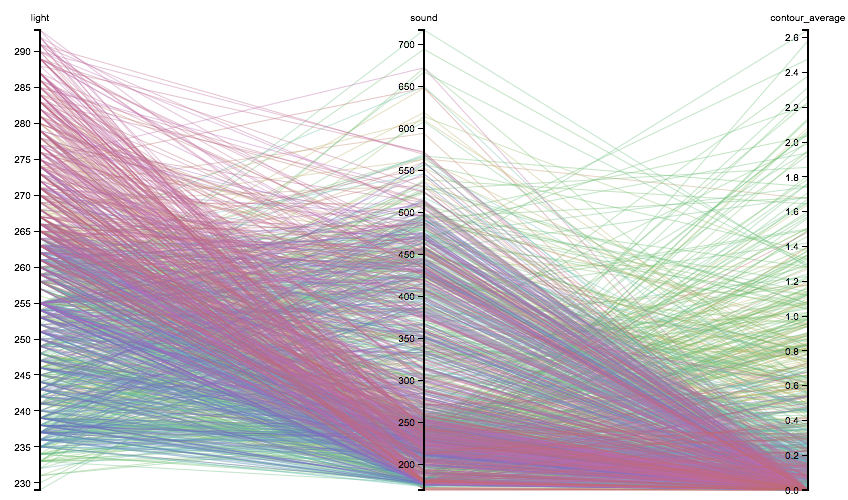
\includegraphics[width=0.97\linewidth]{figs/parallel_cord.png}
    \caption{Parallel coordinates plot for light, sound, and contour average from May 1-2 (a Tuesday and Wednesday). Time of day is represented by color, with reddish-purple being noon and dark blue being midnight. Outliers are excluded from this visualization.}
    \label{fig:pcord}
\end{figure}

\begin{figure}[t]
    \centering
    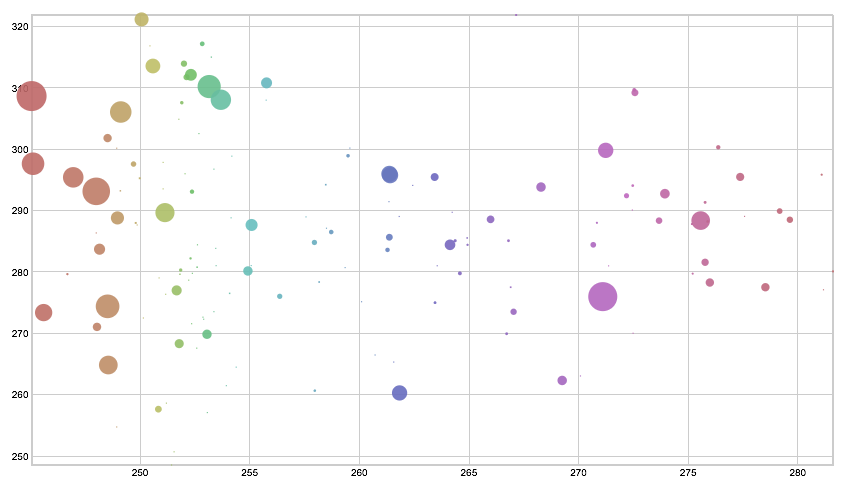
\includegraphics[width=0.97\linewidth]{figs/averages_scatter.png}
    \caption{Scatter plot where each point represents the averaged values for a given hour during the collection period. Light is on the x-axis and sound is on the y-axis. Size represents contour average and color represents time of day (red being day and purple being night). Outliers are excluded from this visualization.}
    \label{fig:scatter}
\end{figure}

\begin{figure}[t]
    \centering
    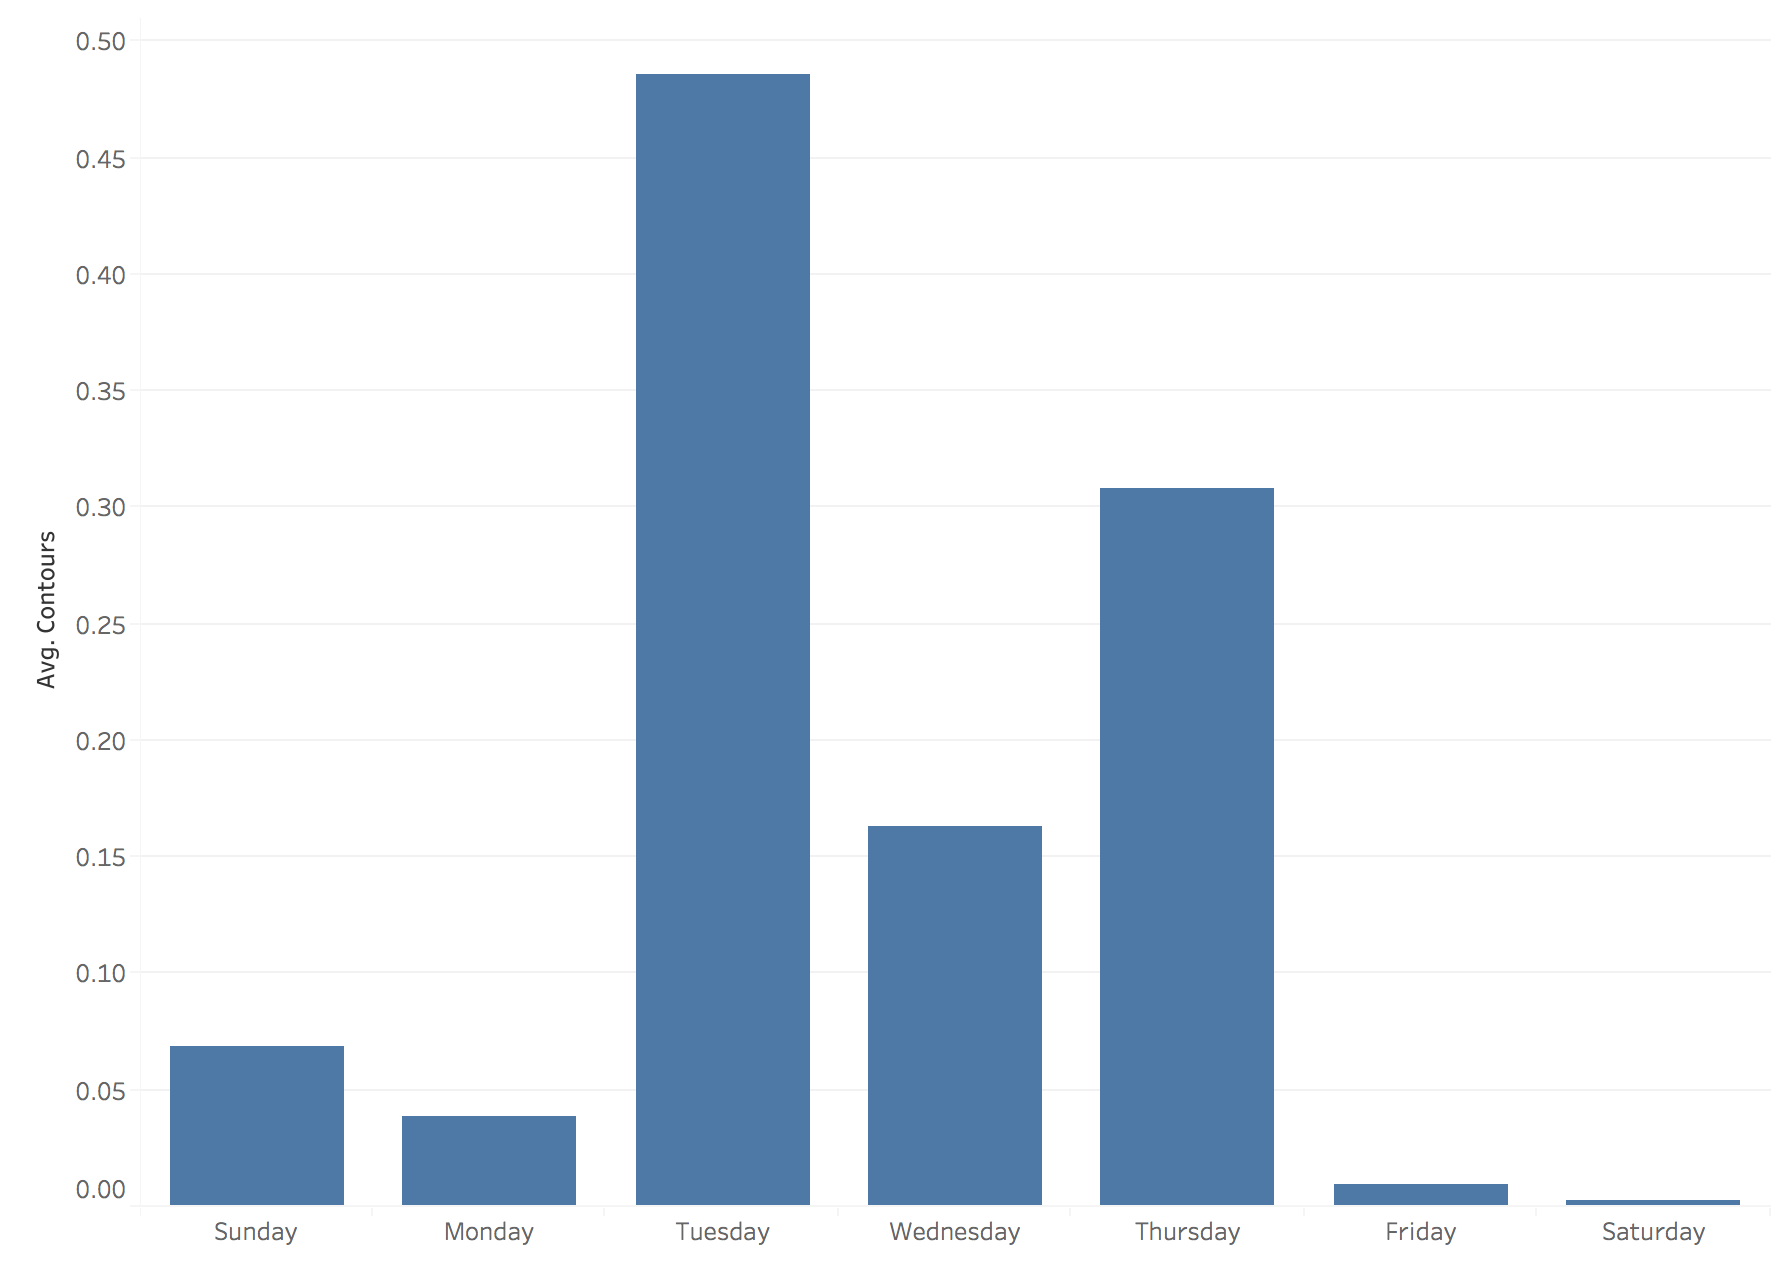
\includegraphics[width=0.97\linewidth]{figs/bars.png}
    \caption{Bar chart showing the average number of contours per minute for each weekday.}
    \label{fig:bars}
\end{figure}